\identify{Identify the Challenge \& Set Goals: MoGo Mechanism (June 15, 2024)}
\label{Identify-the-Challenge-&-Set-Goals:-Clamp}
\chapterauthor{Caleb Bachmeier}
\info{Caleb Bachmeier}{Identify the Challenge \& Set Goals: MoGo}{June 15, 2024}
\textbf{Goal}: We will identify an objective for our robot so that we can address it and build an effective way to pickup stakes
\section*{Problem Statement}
\texthl{We must create a mechanism that effective picks stakes up, so that we can put rings on them.}
\section*{Solution Requirements}
\begin{itemize}
    \item Must only use legal VEX VRC parts
    \item Must fit in the 18" x 18" x 18" cube
    \item Must be able to fit on our drivetrain 
    \item Must use no more than 44 watts (four, eleven watt motors). 
    \item Another, often overlooked, problem is the scarcity of parts, parts are not unlimited. Because of problems at our regular practice place (the place with all of our parts) we must practice elsewhere. Not being able to access  parts is a huge problem.
\end{itemize}
\section*{Solution Goals}
\begin{itemize}
    \item We would love to use pneumatics, so we can use our 22 remaining watts elsewhere.
\end{itemize}
\brainstorm{Brainstorm \& Diagram: MoGo Mechanism (June 17, 2024)}
\label{Brainstorm-&-Diagram:-Clamp}
\chapterauthor{Caleb Bachmeier}
\info{Caleb Bachmeier}{Brainstorm \& Diagram: MoGo}{June 17, 2024}
\textbf{Goal}: Brainstorm our clamp ideas and diagram them
\section*{Possible Solution - MoGo Mechanism}
\noindent
\textbf{Clamp}:

\noindent
\textbf{Pros}:
\begin{itemize}
    \item We would be able use pneumatics 
    \item Very simple design
    \item Very reliable
\end{itemize}
\textbf{Cons}:
\begin{itemize}
    \item If we do use pneumatics, we would have to set up a whole pneumatic system 
    \item It can be complicated to use leverage to clamp the stake down
    \item A clamp would require maintenance 
\end{itemize}

\noindent
\textbf{Forklift}:

\noindent
\textbf{Pros}:
\begin{itemize}
    \item Forklifts can be simpler to design and build compared to complex clamping mechanisms.
    \item A forklift allows you to adjust the height at which you pick up and place rings on the stake. This flexibility can be advantageous for scoring at different levels.
    \item Depending on how you build it, Forklifts typically have a smaller footprint than clamps, leaving more room for other mechanisms on your robot.
\end{itemize}
\textbf{Cons}:
\begin{itemize}
    \item  Ensuring stability while lifting and placing rings can be challenging. The stake may sway or wobble during the process.
    \item Forklifts add weight to the robot, potentially affecting overall performance.
    \item Accurate alignment is crucial for successful ring placement using a forklift.
    \item We could use pneumatics, although it would negate the largest potential benefits.
\end{itemize}
\noindent
\textbf{Scissor Lift}:

\noindent
\textbf{Pros}:
\begin{itemize}
    \item Scissor lifts can extend to various heights, allowing you to reach different levels of the stake.
    \item When compressed, scissor lifts tend to be more stable, making them reliable for lifting rings from lower positions.
    \item Scissor lifts occupy less space compared to some other mechanisms.
\end{itemize}
\textbf{Cons}:
\begin{itemize}
    \item Scissor lifts can be heavy, affecting overall robot performance. Ensuring stability at higher extensions can be challenging.
    \item As the lift extends, it requires more torque to lift the load. This can impact motor efficiency.
    \item Building a stable scissor lift with precise alignment can be intricate.
\end{itemize}

\solution{Choose a Solution \& Make a Plan: MoGo Mechanism (June 23, 2024)}
\label{Choose-a-Solution:-Clamp}
\chapterauthor{Caleb Bachmeier}
\info{Caleb Bachmeier}{Choose a Solution \& Make a Plan: MoGo}{June 23, 2024}
\textbf{Goal}: Choose which solution we will use for our clamp
\section*{Choose a Solution}
\renewcommand{\arraystretch}{1.85} % Change this value as needed
\begin{table}[htb!]
\centering
\begin{tabular}{|>{\centering\arraybackslash}m{1.85cm}|>{\centering\arraybackslash}m{1.85cm}|>{\centering\arraybackslash}m{1.85cm}|>{\centering\arraybackslash}m{1.85cm}|>{\centering\arraybackslash}m{1.85cm}|>{\centering\arraybackslash}m{1.85cm}|>{\centering\arraybackslash}m{1.85cm}|}
\hline
\textbf{Scale 1 - 10} & \textbf{Stability} & \textbf{Simplicity} & \textbf{Cost} & \textbf{Durability} & \textbf{Total} \tabularnewline
\hline
Weight & x3 & x1 & x1 & x2 & \tabularnewline
\hline
Clamp & 10 & 5 & 9 & 10 & 64 \tabularnewline
\hline
Forklift & 6 & 6 & 5 & 6 & 41 \tabularnewline
\hline
Scissor Lift & 6 & 8 & 4 & 4 & 38 \tabularnewline
\hline
\end{tabular}
\caption{Clamp Decision Matrix}
\label{tab:clamp-matrix}
\end{table}
\renewcommand{\arraystretch}{1.85} % Reset to default
Looking at our point totals it would seem that a clamp design would work best for our purpose.
\subsection*{CAD}
\begin{figure}[h!] % Use [hbt!] to place the figures on the same page
    \begin{minipage}{.55\textwidth}
        \centering
        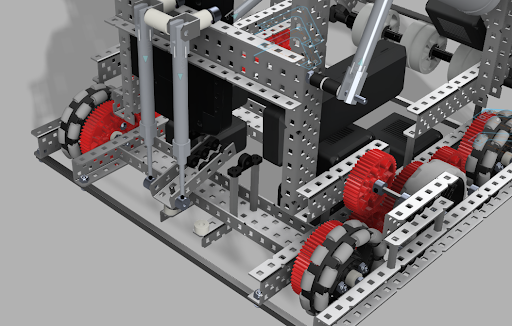
\includegraphics[width=1\linewidth]{images/Iso-Clamp-V1.png}
        \caption{Isometric View}
        \label{fig:iso}
    \end{minipage}
    \begin{minipage}{.55\textwidth}
        \centering
        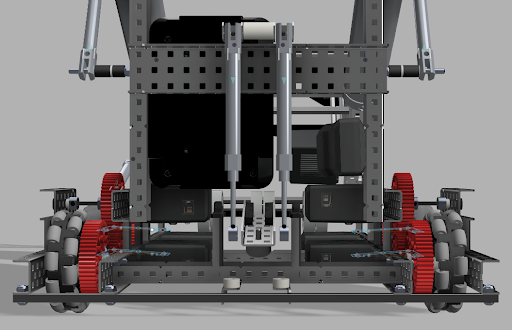
\includegraphics[width=1\linewidth]{images/Front-Clamp-V1.png}
        \caption{Front View}
        \label{fig:front}
    \end{minipage}
    \begin{minipage}{.55\textwidth}
        \centering
        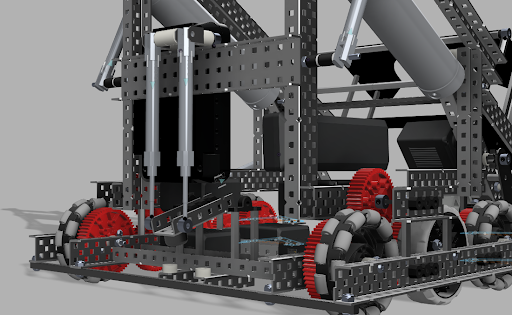
\includegraphics[width=1\linewidth]{images/Side-Clamp-V1.png}
        \caption{Side View}
        \label{fig:side}
    \end{minipage}
    \begin{minipage}{.55\textwidth}
        \centering
        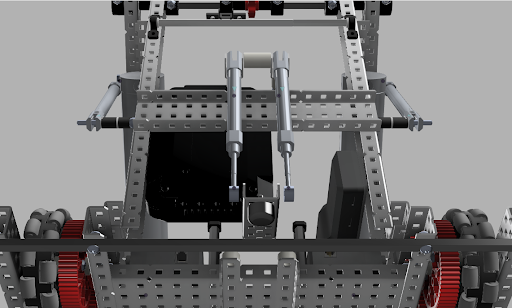
\includegraphics[width=1\linewidth]{images/Bottom-Clamp-V1.png}
        \caption{Bottom View}
        \label{fig:bottom}
    \end{minipage}
\end{figure}

On the following page there are four CAD images describing how we would like to build our clamp. It would use two 55mm stroke double action pistons to push down on the mobile goal and hold it in place. Now it's time to build.
\build{Build: MoGo Mechanism (June 25, 2024)}
\label{Build-&-Program:-Clamp}
\chapterauthor{Caleb Bachmeier}
\info{Caleb Bachmeier}{Build: MoGo}{June 25, 2024}
\textbf{Goal}: Build \& program our selected solution
\section*{Building}
\section*{Initial Concept and Prototype}
One of the first things we did after constructing our drivetrain was design a mobile goal clamp that would allow us to move and score on mobile stakes. Our first design, inspired by our sister team, 7686A, used 2 pistons to pivot C-channels, pressing down and securing a mobile goal. 

Although we designed the concept in CAD before building it, the motion limits within the piston in CAD were far shorter than those on the actual piston. This meant we had to redesign the clamp to work with shorter pistons. Since this was our first prototype and we were eager to see it working, we added spacers to adjust where the pneumatics pivoted on the clamp lever. This version looked rather awkward, but it functioned as expected.

\section*{Reducing Footprint and Design Iteration}
During the construction of our scoring mechanisms, we realized that the current clamp design interfered with the clearance needed by several mechanisms. To reduce the clamp’s footprint, we swapped the original 75mm pistons with 50mm ones, which allowed us to remove the previously added spacers. This provided the necessary clearance for our initial scoring mechanism iterations. However, when we began constructing our first hook intake, we identified the need for further redesign.

\section*{Second-Class Lever Design}
Our new design featured a second-class lever, where the pistons were mounted on the same end that contacted and clamped the mobile goals. We continued using 50mm pistons, but instead of attaching them to the drivetrain base, we mounted them on our intake tower, above the clamp. (See Figure~\ref{fig:lever-design}.) 

Mounting the pistons in this way kept them clear of the inside of the drivetrain, ensuring enough space for the intake chain to pass through. This adjustment significantly improved the integration of our clamp with the rest of the robot.

\section*{Adding Stoppers for Distance and Angle Control}
A major part of our clamp’s functionality was adding stoppers to control how far the mobile goal could enter our robot and at what angle it would sit once clamped. Managing the entry distance was crucial since it determined the clamp’s contact point, directly affecting the grip on the goal. Through testing and incrementally increasing the size of the stoppers on either side of the goal, we found that high-strength shaft collars worked perfectly.

\section*{Angle Control and Hooking Mechanism}
We also needed to control the mobile goal's angle, as it impacted the proximity of the goal’s top to the intake chain. With feedback from 7686A, we determined that the optimal distance was around 2 inches, where the intake hooks would just barely graze the silicone cap when spinning by.

To implement this, we mounted two L-channels just below the clamp’s pivot point. We added a cut low-profile bearing and a spacer, along with a screw, onto each L-channel. This spacer and screw acted as a hook that caught the bottom lip of the mobile goal, preventing it from being removed by opposing teams.

\begin{figure}[h]
    \centering
    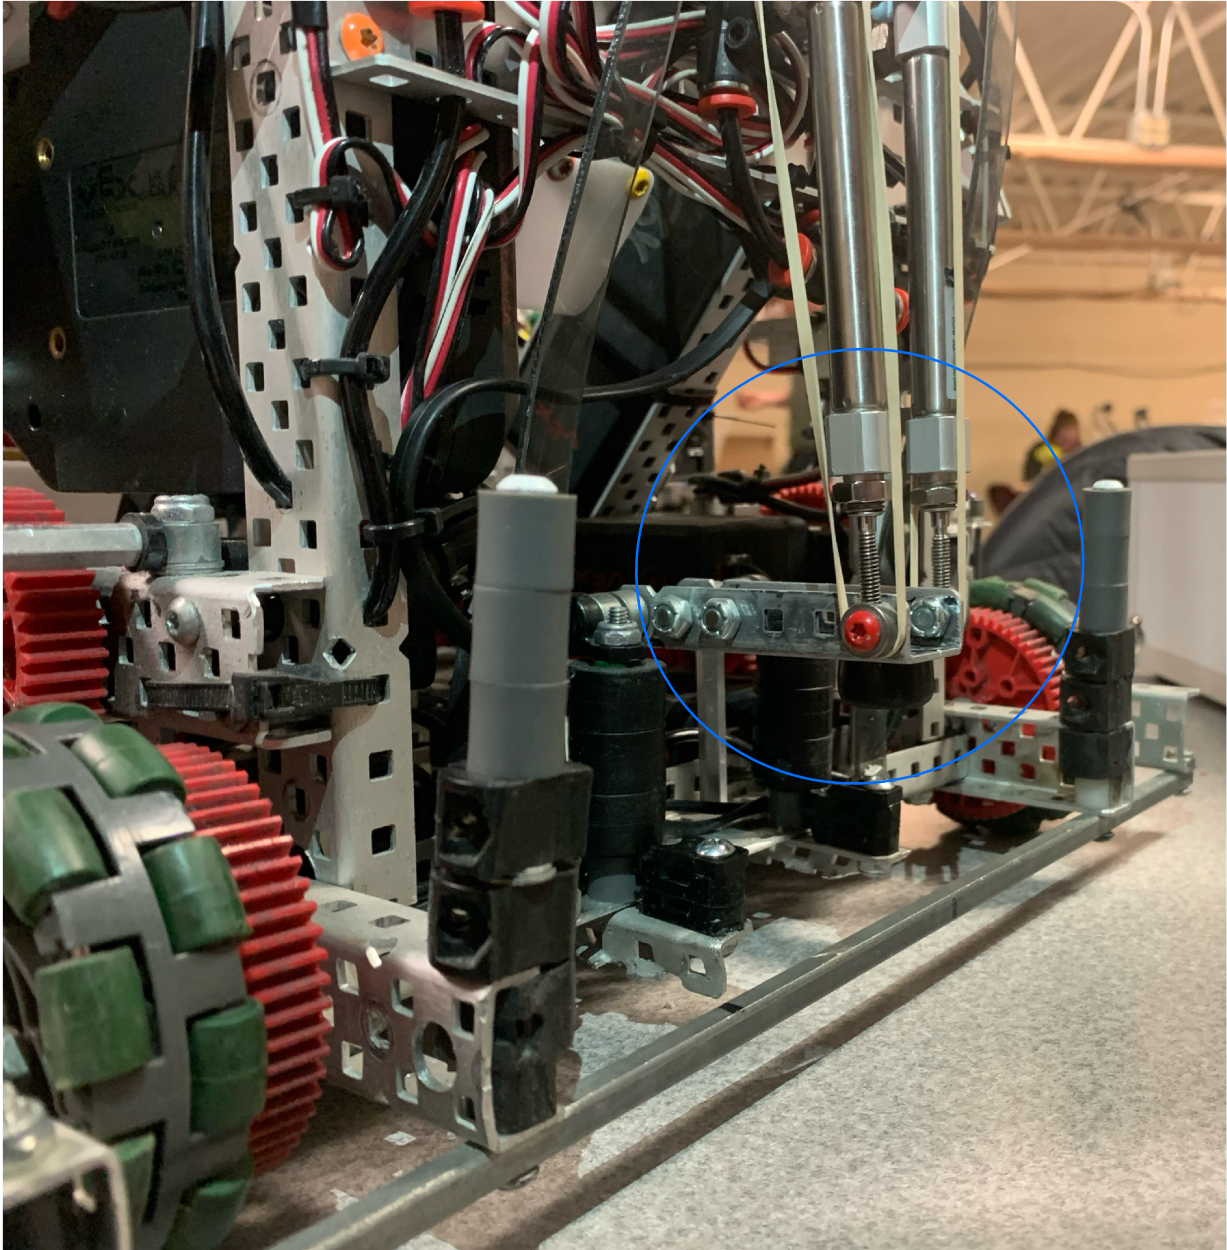
\includegraphics[width=0.8\textwidth]{images/Clamp Lever.jpeg}
    \caption{Second-Class Lever Clamp Design with 50mm Pistons.}
    \label{fig:lever-design}
\end{figure}

\test{Test the Solution: MoGo Mechanism (June 25, 2024)}
\label{Test-the-Solution:-Clamp}
\chapterauthor{Caleb Bachmeier}
\info{Caleb Bachmeier}{Test the Solution: MoGo}{June 25, 2024}
\textbf{Goal}: Test our built solution 
\section*{Test the Solution}
Our clamp has been built and now ready to test, but how should we test it? We thought about using a Spring Scale to measure the force of our pistons, but we already know the force of them; one of our pistons has twelve pounds of force which is approximately 53.4 Newtons of total force, so two pistons would be approximately 106.8 N of force. Then we thought about the force of the Mobile Goal and Rings on the pistons. A Ring weighs 4.3 oz or 122 g. One mobile goal weighs 33.44 oz or 948 g.

So \[1_\text{Ring} \approx 1.196 N\] \[1_\text{Mobile Goal} \approx 9.297 N\] \[2_\text{Pistons} \approx 106.8 N\]

It was then we realized: \[106.8N \text{(The force of our clamp)} > 16.437N\text{(The force of one mobile goal and six rings)}\]

If the force of our clamp was always greater than the force of anything we would need to lift, we wouldn't need the entire 106.8 N of our pneumatics would offer, so as long as our clamp is good enough to lift 16.437 N of force, we should be good.
\section*{Test}
Our test for the clamp is very simple, at which angles could a mobile goal be clamped from? This may sound like an odd question, but it is a very real issue for some teams. This is shown in the image below \\
\begin{figure}[h!]
    \centering
    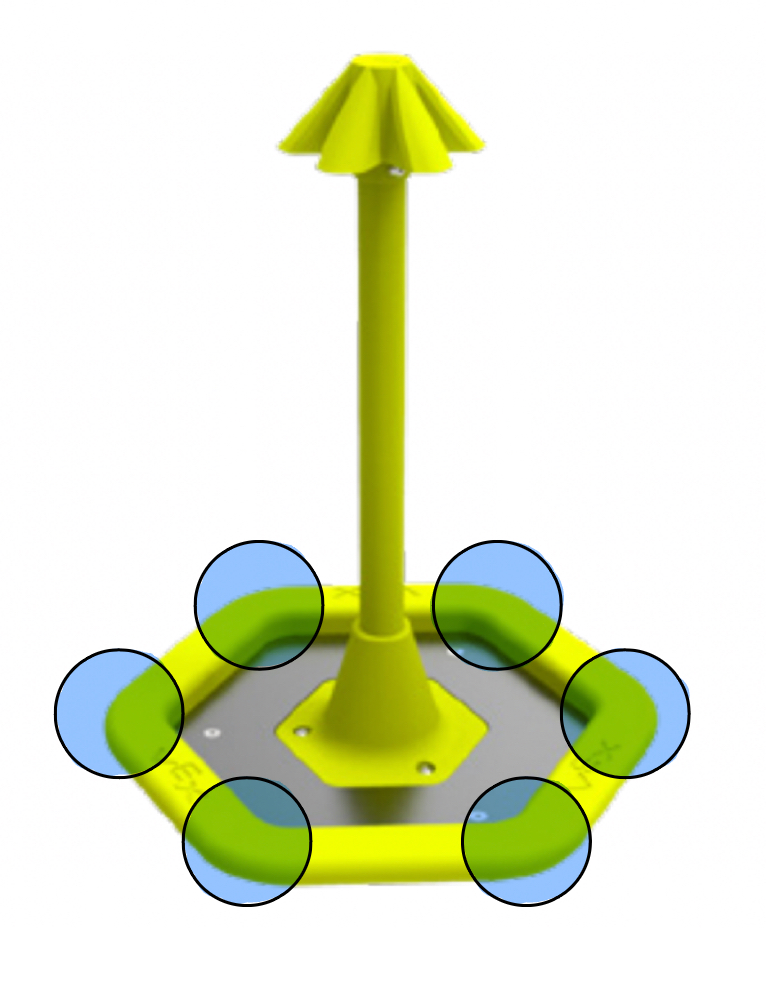
\includegraphics[width=0.5\linewidth]{images/MoGo w Highlights.jpeg}
    \caption{MoGo Issues}
    \label{fig:mogohighlights}
\end{figure}
Some teams have problems clamping onto the mobile goal at these highlighted areas. We need to see if this is a problem for us. \blueref{fig:clamp-v1-corner-test}{(This testing is continued on the next page)}

Another test we need to do is to find the angles at which each mobile goal is clamped down on. We wanted to do this to make sure their weren't any oddities in our data. We used a digital angle finder.
Our data is as follows:
\[
1 \; \text{Mobile Goal} \; + 0 \; \text{Ring} = 7.6 \degree
\]
\[
1 \; \text{Mobile Goal} \; + 1 \; \text{Ring} = 7.6 \degree
\]
\[
1 \; \text{Mobile Goal} \; + 2 \; \text{Ring} = 7.5 \degree
\]
\[
1 \; \text{Mobile Goal} \; + 3 \; \text{Ring} = 7.3 \degree
\]
\[
1 \; \text{Mobile Goal} \; + 4 \; \text{Ring} = 7.2 \degree
\]
\[
1 \; \text{Mobile Goal} \; + 5 \; \text{Ring} = 7.0 \degree
\]
\[
1 \; \text{Mobile Goal} \; + 6 \; \text{Ring} = 6.9 \degree
\]

Our data seems very consistent ranging from 7.6 \degree - 6.9 \degree. This concludes our testing for the clamp, it seems that it was a very good decision and has high build quality. Now time to build our intake mechanism.

\pagebreak

\begin{figure}[h!] % Use [hbt!] to place the figures on the same page
    \begin{minipage}{.5\textwidth}
        \centering
        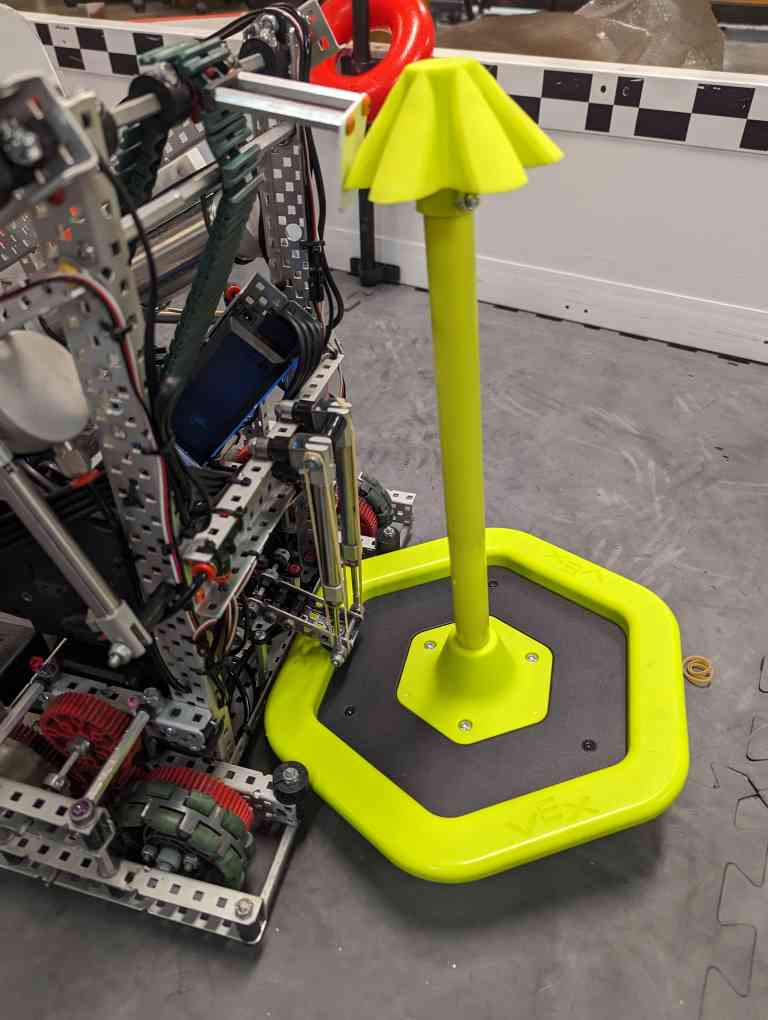
\includegraphics[width=.8\linewidth]{images/Clamp Test V1.jpg}
        \caption{Clamp V1 Test}
        \label{fig:clamp-v1-test}
    \end{minipage}
    \begin{minipage}{.5\textwidth}
        \centering
        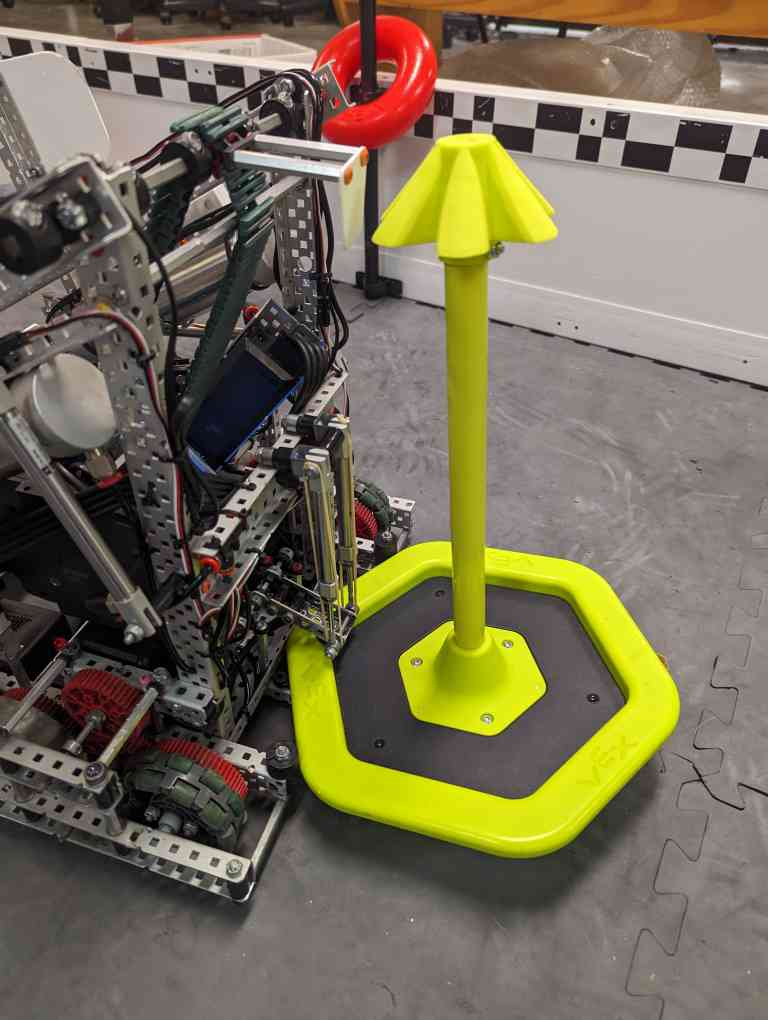
\includegraphics[width=.8\linewidth]{images/Clamp Corner Test V1.jpg}
        \caption{Clamp V1 Corner Test}
        \label{fig:clamp-v1-corner-test}
    \end{minipage}
    \begin{minipage}{.5\textwidth}
        \centering
        \includegraphics[width=.8\linewidth]{images/Clamp Corner Test V1.1.jpg}
        \caption{Clamp V1 Corner Test}
        \label{fig:clamp-v1.1-corner-test}
    \end{minipage}
\end{figure}

These are the tests for our built Clamp, as you can see, in \blueref{fig:clamp-v1-corner-test}{these photos} our test to figure out if we can clamp from the corners is successful. This concludes our testing for the Clamp, it seems to be a very efficient solution for a MoGo mechanism. 